\documentclass[hyperref={pdfpagelabels=false}]{beamer}

\usepackage{listings}
\usepackage{algorithm}
\usepackage{algorithmicx}
\usepackage{algpseudocode}

\usetheme{default}
\setbeamercovered{transparent}
\setbeamertemplate{footline}[page number]
\setbeamertemplate{navigation symbols}{} %remove navigation symbols
\setbeamertemplate{bibliography entry title}{}

\newcommand{\codestyle}{\small\sffamily}

% "define" Scala
\lstdefinelanguage{scala}{
  alsoletter={@,=,>},
  morekeywords={abstract, case, catch, class, def, do, else, extends, false, final, finally, for, if, implicit, import, match, new, null, object, 
override, package, private, protected, requires, return, sealed, super, this, throw, trait, try, true, type, val, var, while, with, yield, domain, 
postcondition, precondition,invariant, constraint, assert, forAll, in, _, return, @generator, ensure, require, holds, ensuring,=>},
  sensitive=true,
  morecomment=[l]{//},
  morecomment=[s]{/*}{*/},
  morestring=[b]"
}
\lstset{
%  frame=tb,
  language=scala,
%  aboveskip=3mm,
%  belowskip=3mm,
%  lineskip=-0.1em,
  showstringspaces=false,
  columns=fullflexible,
  mathescape=true,
  numbers=none,
  numberstyle=\tiny,
  basicstyle=\codestyle
} 

\begin{document}
\title{Toward Interprocedural Pointer and Effect Analysis for Scala}
\author{Etienne Kneuss}
\date{\today}

\nocite{*}

\institute[EPFL]{
Laboratory for Automated Reasoning and Analysis \\
School of Computer and Communication Sciences\\
EPFL\\
\vspace{5pt}
Thesis Supervisor: Viktor Kuncak\\
Thesis Supervisor: Philippe Suter
}

\begin{frame}
    \titlepage
\end{frame}

\section*{Outline}
\begin{frame}
    \frametitle{Outline}
    \tableofcontents
\end{frame}

\section{Introduction}
%\begin{frame}
%    \frametitle{Scala}
%    \begin{itemize}
%        \item Growing language
%        \item Lorem ipsum
%        \item Lorem ipsum
%    \end{itemize}
%\end{frame}

\begin{frame}[label=overview]
%    \frametitle{INSANE}
    \begin{figure}[t]
        
\includegraphics[width=60mm]{../../logo.png}\\
        Interprocedural Static Analysis Engine for Scala
    \end{figure}

    \begin{itemize}
        \item Precise pointer and effect analysis
            \begin{itemize}
                \item Whole-Program but compositional
                \item Based on abstract interpretation
                \item Interprocedural
            \end{itemize}
        \item Working Implementation
            \begin{itemize}
                \item Provided as a compiler plug-in
                \item Accepts any Scala code
                \item Requires no annotations
            \end{itemize}
    \end{itemize}
\end{frame}

\begin{frame}
\frametitle{Definitions}
    \textbf{Pointer Analysis}\\
    \emph{Static analysis technique that builds information on the
relations between pointers and allocated objects.}

    \vspace{30pt}

    \textbf{Effect Analysis}\\
    \emph{Static analysis technique that summarizes the side effects
of procedures in a certain domain.}
\end{frame}

\section{Analysis}
\begin{frame}
    \frametitle{Analysis Phases}
    The analysis currently consists of five main phases:
    \begin{enumerate}
        \item \textcolor{gray}{Abstract Syntax Tree Extraction}
        \item \textcolor{gray}{Control Flow Graphs Generation}
        \item Class Analysis \& Call Graph Generation
        \item Effect Graphs Generation
        \item Purity Analysis
    \end{enumerate}
\end{frame}

\subsection{Class Analysis}
\begin{frame}[fragile]
\frametitle{Class Analysis}

    Class Analysis aims at establishing the types of runtime values. In
    the presence of dynamic dispatch, this information is used to compute a
    precise call-graph.

    \begin{columns}
      \begin{column}{0.5\textwidth}
\begin{lstlisting}
object Test {
    def run1(obj: A) {
        obj.f()
    }
    def run2() {
        val obj = new A
        obj.f()
    }
}
\end{lstlisting}
      \end{column}
      \begin{column}{0.5\textwidth}
\begin{lstlisting}
class A {
    def f() { ... }
}
class B extends A {
    def f() { ... }
}
\end{lstlisting}
      \end{column}
    \end{columns}


\end{frame}

\begin{frame}[fragile]
    \frametitle{Class Analysis}
    \begin{itemize}
        \item Analysis is flow sensitive, based on abstract interpretation
        \item For each local variable, we assign an abstract value of the form:
        $$ \langle T_{sub}, T_{exact} \rangle $$ where $T_{sub}$ and
        $T_{exact}$ are two sets of types
    \end{itemize}

\begin{figure}
    \begin{tabular}{ l | l }
        Expression $ex$       & Abstract Value $\alpha(ex)$\\
        \hline
        \verb/new A/          & $\langle \emptyset, \{ A \} \rangle$ \\
        \verb/null/           & $\langle \emptyset, \emptyset \rangle$ \\
        \verb/obj.f/          & $\langle\{type(\verb/obj.f/)\}, \{type(\verb/obj.f/)\} \rangle$ \\
        \verb/rec.meth(..)/   & $\langle\{type(\verb/rec.meth/)\}, \{type(\verb/rec.meth/)\} \rangle$ \\
    \end{tabular}
\end{figure}
\end{frame}

\begin{frame}[fragile]
    \frametitle{Class Analysis}
    Once we collected type information for every local variables, we generate
    the call graph.

    In the presence of a call \lstinline{rec.meth()}, with
    $\langle T_{sub}, T_{exact} \rangle$ as type information for \lstinline{rec},
    we consider calls to:
    $$
    \{ C.meth ~|~ (C \in T_{exact} \lor C \sqsubset T_{sub}) \land meth \in declMethods(C)\}
    $$

    The call graph is then used to compute sets of mutually-dependant
    procedures (strongly connected components), and then to order the effect
    analysis (topological sort).
\end{frame}

\subsection{Effect/Alias Analysis}
\begin{frame}
    \frametitle{Effect/Alias Analysis}
    \begin{itemize}
        \item Analysis based on abstract interpretation
        \item Graphs as representation
        \item Compositional: One graph per method, with "connecting" nodes.
    \end{itemize}

    Graphs are defined as:
    \begin{eqnarray*}
        G           := &\langle& N \subseteq Nodes, \\
                       && E \subseteq Edges, \\
                       && locVar \subseteq Variables \times \mathcal{P}(N), \\
                       && RetNodes \subseteq N \rangle \\
    \end{eqnarray*}
%    \begin{figure}[t]
%        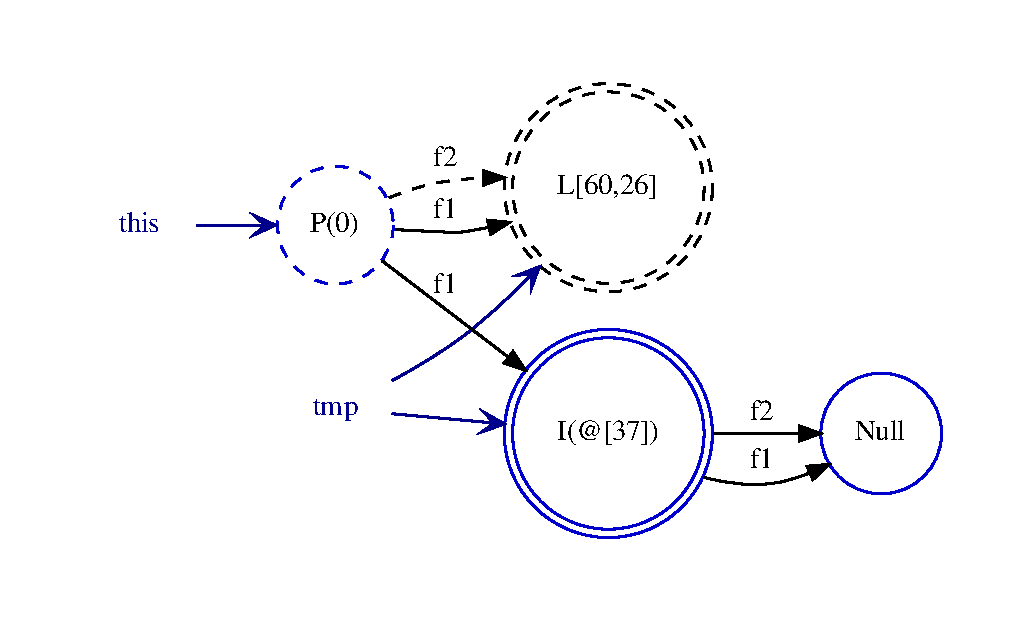
\includegraphics[width=80mm]{images/pt_graph1.pdf}\\
%    \end{figure}
\end{frame}

\begin{frame}
    \frametitle{Graph Semantics}
    \framesubtitle{Nodes}

    \begin{itemize}
        \item We define different kinds of nodes:
            \begin{itemize}
                \item Inside Nodes (INodes) represent allocated objects.
                \item Parameter Nodes (PNodes) represent the current object
                    (\lstinline{this}) as well as the method parameters.
                \item Load Nodes (LNodes) represent nodes that are not yet
                    fully determined.
                \item Object Nodes (OBNodes) represent global objects,
                    constructed using the \lstinline{object} Scala construct.
                \item Null Node (NNode) represents the special
                    \lstinline{null} value.
                \item Literal Nodes represent literals of primitive types, such as
                    int, boolean or string
            \end{itemize}
        \item We also use the following conventions:
            \begin{itemize}
                \item Nodes that are returned from the procedure have a double
                border.
                \item Nodes that represent singleton objects are drawn in
                blue.
            \end{itemize}
    \end{itemize}
\end{frame}

\begin{frame}
    \frametitle{Graph Semantics}
    \framesubtitle{Nodes}
    \begin{figure}[t]
        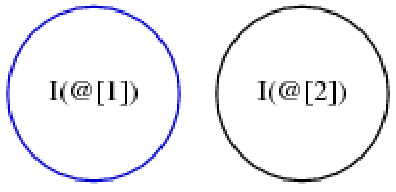
\includegraphics[width=40mm]{images/nodes/inodes.pdf}
    \end{figure}
    \begin{figure}[t]
        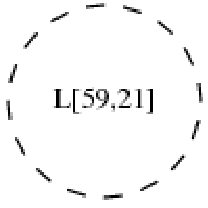
\includegraphics[width=15mm]{images/nodes/lnodes.pdf}
        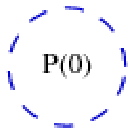
\includegraphics[width=10mm]{images/nodes/pnodes.pdf}
        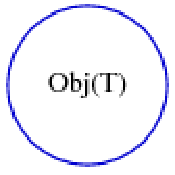
\includegraphics[width=15mm]{images/nodes/objnodes.pdf}
    \end{figure}
    \begin{figure}[t]
        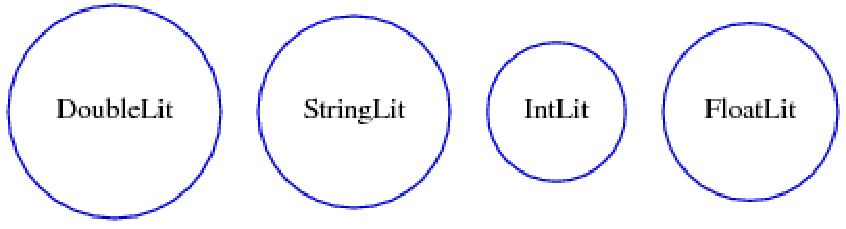
\includegraphics[width=60mm]{images/nodes/litnodes.pdf}
    \end{figure}
\end{frame}

\begin{frame}
    \frametitle{Graph Semantics}
    \framesubtitle{Edges}

    \begin{itemize}
        \item \textbf{Inside Edges} represent write operations on the
        corresponding fields, they are represented as full edges, with the
        field's name as label.
        \begin{figure}[t]
            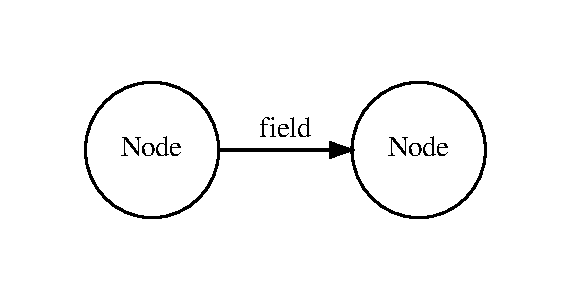
\includegraphics[width=40mm]{images/nodes/iedge.pdf}
        \end{figure}

        \item \textbf{Outside Edges} represent the path to follow to reach
        \emph{load nodes}. They are represented as dashed edges, with the
        field's name as label.
        \begin{figure}[t]
            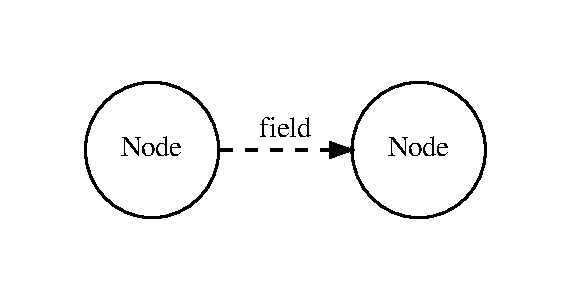
\includegraphics[width=40mm]{images/nodes/oedge.pdf}
        \end{figure}
    \end{itemize}
\end{frame}

\begin{frame}[fragile]
    \frametitle{Graph Semantics}
    \framesubtitle{Example}
    \begin{columns}
      \begin{column}{0.4\textwidth}
\begin{lstlisting}
class T(var f1: T, var f2: T) {
  def test() = {
    var tmp = this.f2
    if (tmp != null) {
      tmp = new T(null, null)
    }
    this.f1 = tmp
    tmp
  }
}
\end{lstlisting}
      \end{column}
      \begin{column}{0.7\textwidth}
        \begin{figure}[t]
            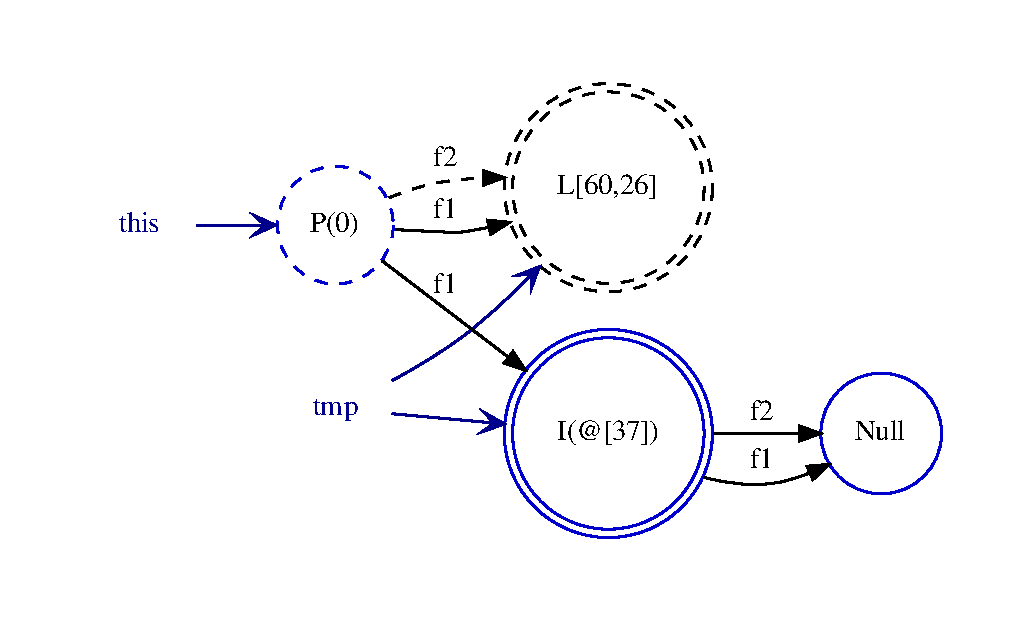
\includegraphics[width=80mm]{images/pt_graph1.pdf}\\
        \end{figure}
      \end{column}
    \end{columns}
\end{frame}

\begin{frame}[fragile]
    \frametitle{Effects Analysis}
    \framesubtitle{Transfer function}

        \begin{tabular}{ l | l }
            Statement $st$                & Transfer Function \emph{f}\\
            \hline
            \verb/r = v/                     & $\langle N, E, locVar[r \mapsto locVar(v)], R \rangle$ \\
            \verb/r = new C/ @p              & $alloc(G, r, C, @p)$ \\
            \verb/r = null/                  & $\langle N \cup \{NNode\}, E,$ \\
                                             & $~~ locVar[r \mapsto \{ NNode \}], R \rangle$ \\
            \verb/r.f = v/ @p                & $write(G, locVar(r), f, locVar(v), @p)$ \\
            \verb/r = v.f/ @p                & $read(G, locVar(v), f, r, @p)$ \\
            \verb/r = v.meth(a1, .., an)/ @p & $call(G, r, v, meth, (a_1, ..., a_n), @p)$ \\
            \verb/return v/                  & $\langle N, E, locVar, locVar(v) \rangle$ \\
        \end{tabular}
\end{frame}

\begin{frame}[fragile]
    \frametitle{Effects Analysis}
    \framesubtitle{Allocations}
    We use allocation site abstraction
        \begin{itemize}
            \item One node per program point
            \item We need to determine if this node might represent multiple
                objects
            \item We detect loops around allocation sites
        \end{itemize}
    \begin{columns}
      \begin{column}{0.3\textwidth}
\begin{lstlisting}
    def test() {
        var a = null
        while(..) {
            a = new A
        }
    }
\end{lstlisting}
      \end{column}
      \begin{column}{0.7\textwidth}
        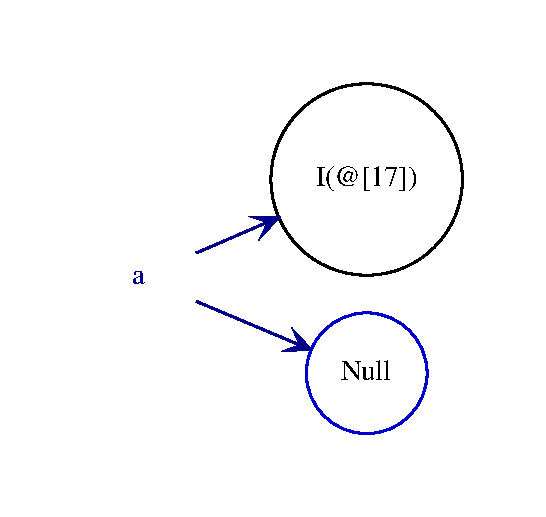
\includegraphics[width=60mm]{images/alloc.pdf}
      \end{column}
    \end{columns}
\end{frame}

\begin{frame}[fragile]
    \frametitle{Effects Analysis}
    \framesubtitle{Field Reads}
    When analyzing a field read, we have two cases:
    \begin{enumerate}
        \item The targeted nodes are already determined, and we simply use them
        \item The targeted nodes are not determined, we need to introduce a
        load node
    \end{enumerate}
    \begin{columns}
      \begin{column}{0.4\textwidth}
\begin{lstlisting}
    class A(var f1: A, var f2: A) {
        def test() {
            this.f1 = null
            val v1 = this.f1
            val v2 = this.f2
        }
    }
\end{lstlisting}
      \end{column}
      \begin{column}{0.6\textwidth}
        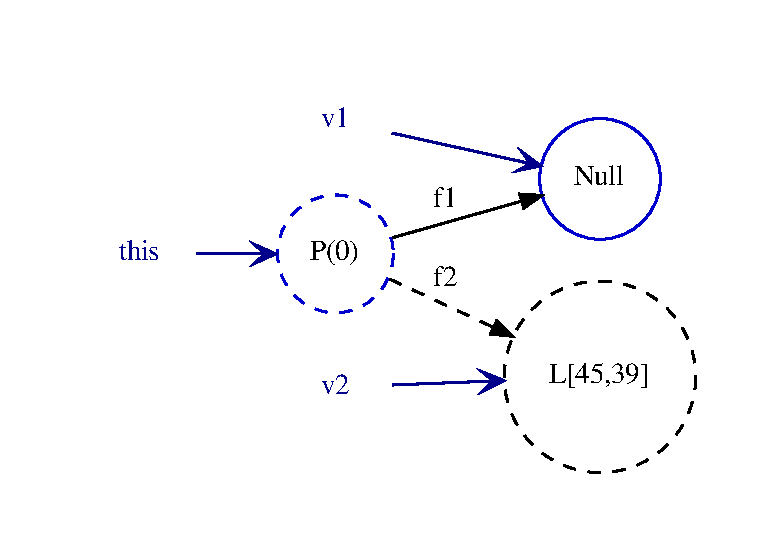
\includegraphics[width=60mm]{images/reads.pdf}
      \end{column}
    \end{columns}
\end{frame}

\begin{frame}[fragile]
    \frametitle{Effects Analysis}
    \framesubtitle{Field Writes}

    \textbf{Strong/Weak Update} \\
    \emph{ When a field update completely overwrites the old value, it is said
    to be \textbf{strong}.}

    \vspace{10pt}

    One variable may represent multiple objects, we thus cannot always do
    strong updates. The criteria for a strong update on \lstinline{obj.f = v}
    is
    $$|locVar(obj)| = 1 \land \forall n \in locVar(obj) ~.~ n.isSingleton$$

    \begin{columns}
      \begin{column}{0.4\textwidth}
\begin{lstlisting}
    class A(var f: A) {
        def test(a1: A, a2: A) {
            val o = if (..) a1 else a2
            a1.f = null
            o.f  = null
        }
    }
\end{lstlisting}
      \end{column}
      \begin{column}{0.5\textwidth}
        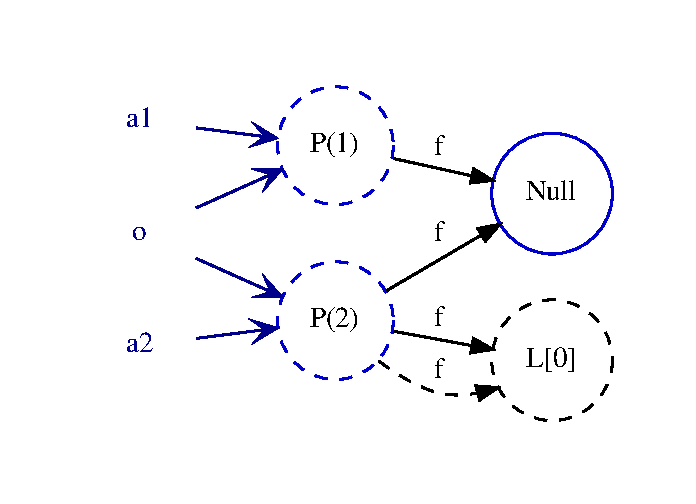
\includegraphics[width=50mm]{images/writes.pdf}
      \end{column}
    \end{columns}
\end{frame}

\begin{frame}[fragile]
    \frametitle{Join Operation}

    We need to take specific care when joining back two branches:
    \begin{itemize}
        \item Write operations that occur only on one branch are similar to
        weak updates.
        \item As usual, if no old value is found, we introduce a load node
    \end{itemize}

    \begin{columns}
      \begin{column}{0.4\textwidth}
\begin{lstlisting}
    class A(var f: A) {
        def test(a1: A, a2: A) {
            if (..) {
                a1.f = null
            } else {
                a2.f = null
            }
        }
    }
\end{lstlisting}
      \end{column}
      \begin{column}{0.6\textwidth}
        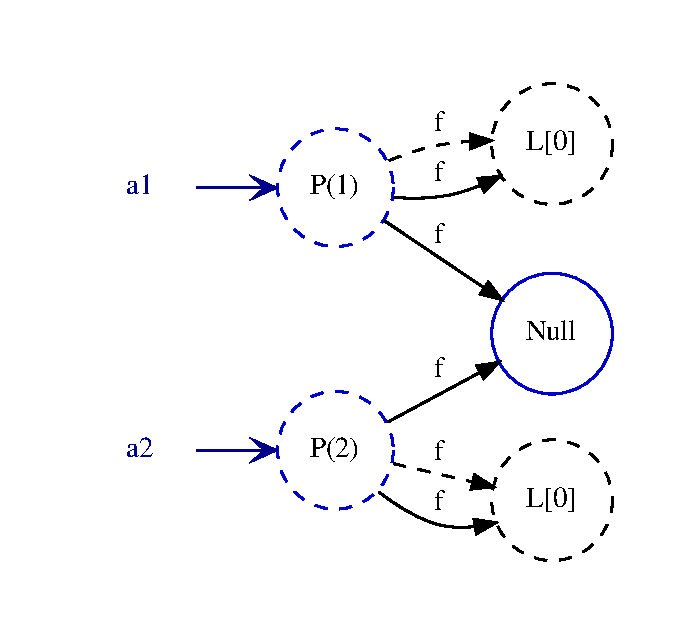
\includegraphics[width=50mm]{images/join.pdf}
      \end{column}
    \end{columns}
\end{frame}

\begin{frame}[fragile]
    \frametitle{Method Inlining}
    To analyze the effects of a function call, we need to \emph{inline} the
    callee into the caller.

    \vspace{10pt}

    This inlining is made of two steps:
    \begin{itemize}
        \item Map nodes from the callee to the caller
        \item Apply write operations
    \end{itemize}

\begin{columns}
      \begin{column}{0.40\textwidth}
\begin{lstlisting}
class A {
  var f: A = null
  def test(a1: A, a2: A, a3: A) {
    a2.f = this.f
    a1.f = a2
    a1.f = a3
  }

\end{lstlisting}
      \end{column}
      \begin{column}{0.60\textwidth}
\begin{lstlisting}
  def plop() {
    val o1 = new A
    val o2 = new A
    val o3 = if (this!=null) o1 else o2
    o1.test(o3, o2, o2)
  }
}
\end{lstlisting}
      \end{column}
\end{columns}
\end{frame}

\begin{frame}[fragile]
    \frametitle{Method Inlining}
    \framesubtitle{Mapping Nodes}

    \begin{itemize}
        \item First parameter node is mapped to the receiver
        \item Other parameter nodes are mapped to nodes passed as argument at
        the call site
        \item Inside node are mapped to themselves, but with a composed program
        point.
        \item Load nodes are mapped by following first inside and then outside
        edges.
        \item Literal and object nodes are mapped to themselves.
        \item Return nodes are mapped to the node presenting the return value.
    \end{itemize}


\end{frame}


\begin{frame}[fragile]
    \frametitle{Method Inlining}
    \framesubtitle{Mapping Nodes}

    \begin{center}
        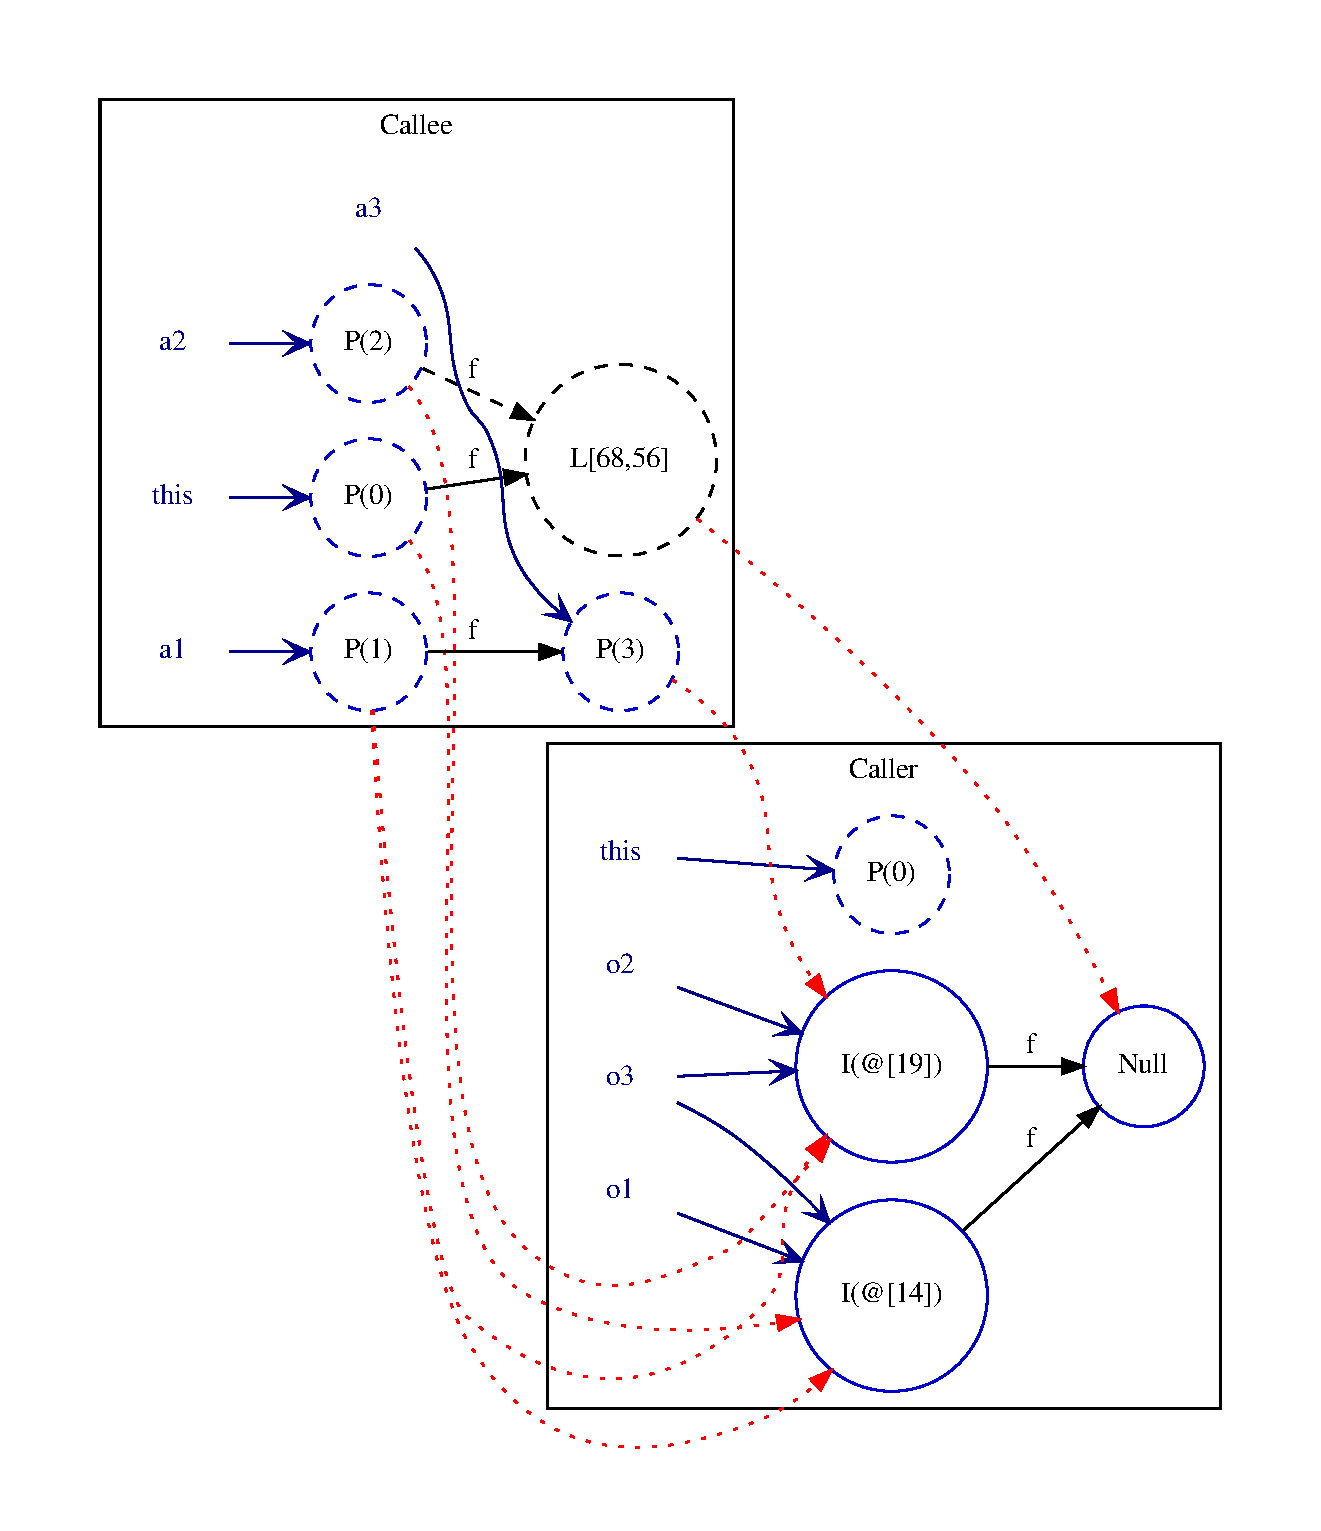
\includegraphics[width=70mm]{images/pt_map1.pdf}
    \end{center}
\end{frame}

\begin{frame}[fragile]
    \frametitle{Method Inlining}
    \framesubtitle{Applying Writes}

    \begin{itemize}
        \item In the callee graph, we have no information about the order in
        which write operations are performed.
        \item We thus apply write operations until the graph reaches a
        fix-point.
    \end{itemize}

    \vspace{15pt}
    \textbf{Inlining Result:}
    \begin{center}
        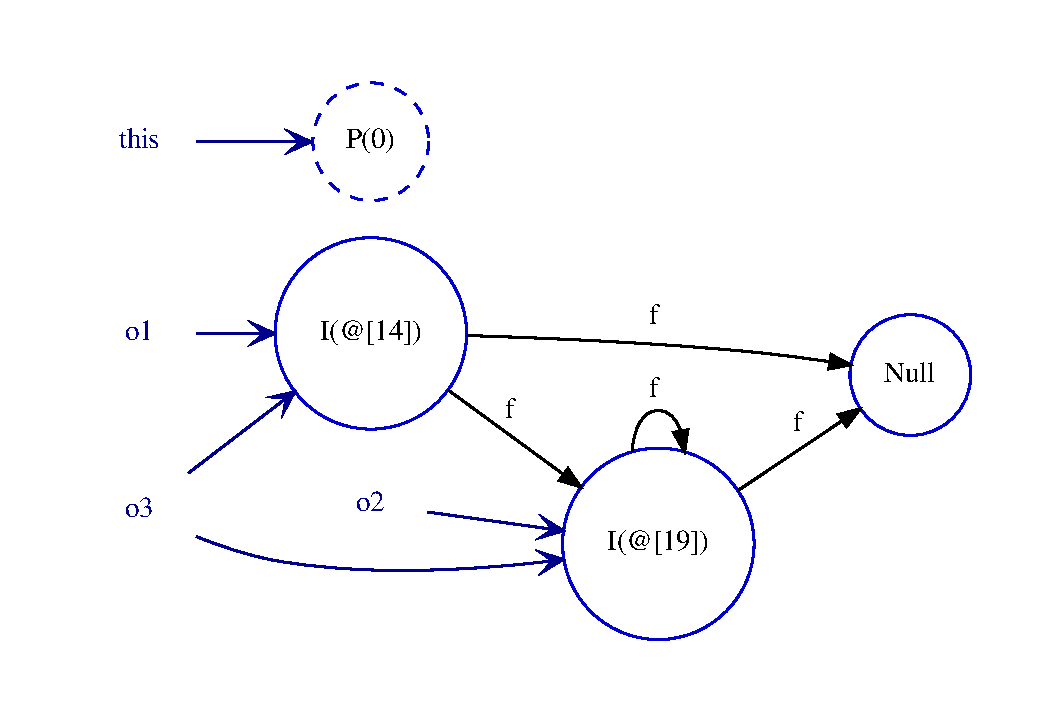
\includegraphics[width=70mm]{images/pt_inline1result.pdf}
    \end{center}
\end{frame}

\subsection{Purity Analysis}
\begin{frame}[fragile]
    \frametitle{Purity Analysis}
    \begin{itemize}
        \item We check for \emph{observable} purity
            \begin{itemize}
                \item Look for inside edges (writes) reachable from nodes
accessible from \emph{outside} (PNodes, OBNodes, ...)
            \end{itemize}
        \item If not pure, we compute \emph{modifies clauses}
    \end{itemize}

    \begin{columns}
      \begin{column}{0.5\textwidth}
\begin{lstlisting}
class Counter {
  var v = 0
}

class Test1 {
  def fun() {
    val localC = new Counter
    localC.v = 42
  }
}
\end{lstlisting}
      \end{column}
      \begin{column}{0.5\textwidth}
\begin{lstlisting}
class Test2 {
  val c = new Counter
  def fun() {
    c.v = 42
  }
}
\end{lstlisting}
      \end{column}
    \end{columns}
\end{frame}

\begin{frame}[fragile]
    \frametitle{Purity Analysis}
    \begin{columns}
      \begin{column}{0.4\textwidth}
\begin{lstlisting}
class Test1 {
  def fun() {
    val localC = new Counter
    localC.v = 42
  }
}
\end{lstlisting}
        \uncover<2->{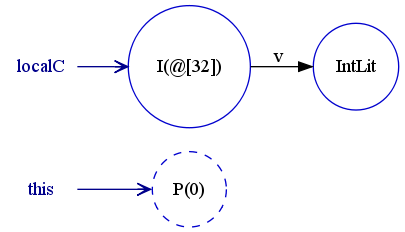
\includegraphics[width=40mm]{images/purity_fun1_pt.png}}
        \uncover<2->{\vspace{10pt}}
        \uncover<2->{\lstinline{Test1.fun: Pure}}
      \end{column}
      \begin{column}{0.6\textwidth}
\begin{lstlisting}
class Test2 {
  val c = new Counter
  def fun() {
    c.v = 42
  }
}
\end{lstlisting}
        \uncover<2->{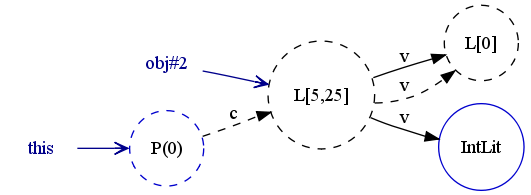
\includegraphics[width=50mm]{images/purity_fun2_pt.png}}
        \uncover<2->{\vspace{10pt}}
        \uncover<2->{\lstinline{Test2.fun: Modifies(this.c.v)}}
      \end{column}
    \end{columns}
\end{frame}

\section{Implementation}
\begin{frame}[fragile]
    \frametitle{Implementation}
    \begin{itemize}
        \item Implemented as a Scala compiler plug-in
        \item Database storage for:
        \begin{itemize}
            \item Class Hierarchy
            \item Intermediate  graphs
        \end{itemize}
        \item Specifying unanalyzable methods:
        \begin{lstlisting}
@AbstractsClass("java.lang.Long")
class javalangLong {
  @AbstractsMethod("java.lang.Long.hashCode(()Int)")
  def __hashCode(): Int = {
    42
  }
}
        \end{lstlisting}
    \end{itemize}

\end{frame}

\begin{frame}
    \frametitle{Implementation}
    \framesubtitle{Difficulties}
    \begin{itemize}
        \item Our phase is late in the compiling process: code has been
        expanded/rewritten.

        \item No trivial way to access the class hierarchy, required for
        generating the call graph.

        \item Compiler becomes brittle for tasks out of its initial scope.

        \item Dependencies to the Java library are unanalyzable.

        \item Custom serialization procedure is required to store compiler
        objects in a database.
    \end{itemize}

\end{frame}

\section{Conclusion}
\subsection{Limitations and Future Work}
\begin{frame}
\frametitle{Limitations and Future Work}
    \begin{itemize}
        \item Exceptions
        \begin{itemize}
            \item Simple but unsound handling
            \item Require some further analysis to handle them correctly without
cluttering the CFG.
        \end{itemize}
        \item Concurrency
        \begin{itemize}
            \item No support
            \item Scala encourages concurrency based on message-passing (actors)
        \end{itemize}
        \item Higher order functions
        \begin{itemize}
            \item Currently very imprecise
            \item Possible solution: graph-based delaying of method calls
        \end{itemize}
        \item Annotations
        \begin{itemize}
            \item Support for more annotations
        \end{itemize}
    \end{itemize}
\end{frame}

\subsection{Related Work}
\begin{frame}[allowframebreaks]
    \frametitle{Related Work}
    \bibliographystyle{alpha}
    \bibliography{slides.bib}
\end{frame}

\againframe{overview}

%\usebackgroundtemplate{
\includegraphics[width=\paperwidth, height=\paperheight]{images/rolex.jpg}}
%\setbeamercolor{title}{parent=palette tertiary} 

\section*{Thanks}
\begin{frame}
    \frametitle{Thanks}
    \begin{center}
        \vspace{-40pt}
        \textbf{Questions ?}
    \end{center}
\end{frame}

\usebackgroundtemplate{}

\appendix
\newcounter{finalframe}
\setcounter{finalframe}{\value{framenumber}}

\setbeamercolor{normal text}{bg=black}

\begin{frame}
\end{frame}

\setbeamercolor{normal text}{bg=white}

\begin{frame}
    \begin{center}
        \textbf{Additional Material}
    \end{center}
\end{frame}


\begin{frame}[fragile]
    \frametitle{Class Analysis}
    \framesubtitle{Transfer Function}

    \begin{figure}
        \begin{tabular}{ l | l }
            Statement             & Transfer Function\\
            \hline
            \verb/v1 = v2/        & $facts = facts[v1 \mapsto facts[v2]]$ \\
            \verb/v1 = ex/        & $facts = facts[v1 \mapsto \alpha(ex)]$ \\
            \verb/obj.f = ex/     & \emph{ignore} \\
            \verb/.../            & \emph{ignore} \\
        \end{tabular}
    \end{figure}

    \begin{figure}
        \begin{tabular}{ l | l }
            Expression $ex$       & Abstract Value $\alpha(ex)$\\
            \hline
            \verb/new A/          & $\langle \emptyset, \{ A \} \rangle$ \\
            \verb/null/           & $\langle \emptyset, \emptyset \rangle$ \\
            \verb/obj.f/          & $\langle\{type(\verb/obj.f/)\}, \{type(\verb/obj.f/)\} \rangle$ \\
            \verb/rec.meth(..)/   & $\langle\{type(\verb/rec.meth/)\}, \{type(\verb/rec.meth/)\} \rangle$ \\
        \end{tabular}
    \end{figure}
\end{frame}

\begin{frame}[fragile,shrink=20]
    \frametitle{Effect Analysis}
    \begin{algorithm}[H]
    \caption{Lattice Join Operation}\label{algo:pt:join}
    \begin{algorithmic}[1]
    \Function{$\bigsqcup$}{$graphs = \{G_1, .., G_n\}$}
        \If{$|graphs| = 1$}
            \State \Return $x \textsf{ s.t. } x \in graphs$
        \Else
            \State $N_{common} \gets \bigcap_i N_i$
            \State $Pairs_{all} \gets  \bigcup_i \{ \langle ie.v1, ie.f \rangle ~|~ ie \in G_i.E \land ie \textsf { is IEdge}\}$
            \State $Pairs_{common} \gets  \bigcap_i \{ \langle ie.v1, ie.f \rangle ~|~ ie \in G_i.E \land ie \textsf { is IEdge}\}$
            \State $N_{load} \gets \{ safeLNode(p.v1, p.f, @0) ~|~ p \in Pairs_{all} - Pairs_{common} \land p.v1 \in N_{common} \}$
            \State $E_{load} \gets \{ IEdge(in.v1, in.f, in) ~|~ in \in N_{load} \} \cup \{ OEdge(in.v1, in.f, in) ~|~ in \in N_{load} \}$
            \State \Return $\langle \bigcup_i G_i.N \cup N_{load}, \bigcup_i G_i.E \cup E_{load}, \bigcup_i G_i.locVar , \bigcup_i G_i.R \rangle$
        \EndIf
    \EndFunction
    \end{algorithmic}
    \end{algorithm}
\end{frame}

\begin{frame}[fragile]
    \frametitle{Effect Analysis}
    \framesubtitle{Types associated to nodes}

    \begin{figure}[h]
        \centering

        \begin{tabular}{ l | l }
            Node Type & Types Associated \\
            \hline
            INode(A)           & $\langle \emptyset, \{A\}\rangle$ \\
            LNode(a, f)        & $\langle\{type(a.f)\}, \{type(a.f)\}\rangle$ \\
            PNode(arg)         & $\langle\{type(arg)\}, \{type(arg)\}\rangle$ \\
            OBNode(A)          & $\langle \emptyset,   \{A\}\rangle$ \\
            NNode              & $\langle \emptyset,   \emptyset \rangle$ \\
            GBNode             & $\langle\{Object\},   \{Object\}\rangle$ (all)\\
            Literal Nodes      & $\langle \emptyset,   \{type(Literal)\}\rangle$\\
        \end{tabular}
    \end{figure}

\end{frame}

\begin{frame}[fragile,shrink=20]
    \frametitle{Effect Analysis}
    \begin{algorithm}[H]
    \caption{Allocations}\label{algo:pt:alloc}
    \begin{algorithmic}[1]
    \Function{alloc}{$\langle N, E, locVar, R \rangle, r, C, @p$}
        \State $n       \gets INode(C, false, @p)$
        \State $n_{sgt} \gets INode(C, true, @p)$

        \If{$n_{sgt} \in N$}
            \State $N_{new} \gets (N \cup \{ n \}) - \{ n_{sgt} \}$
            \State $locVar_{new} \gets \{ v \mapsto v_{nodes}[n_{sgt} \mapsto n] ~|~ (v \mapsto v_{nodes}) \in locVar \}$
            \State $locVar_{new} \gets locVar_{new}[ r \mapsto \{n\}]$
        \Else
            \State $N_{new} \gets N \cup \{ n_{sgt} \}$
            \State $locVar_{new} \gets locVar[ r \mapsto \{n_{sgt}\}]$
        \EndIf
        \State \Return $\langle N_{new}, E, locVar_{new}, R \rangle$
    \EndFunction
    \end{algorithmic}
    \end{algorithm}
\end{frame}

\begin{frame}[fragile,shrink=40]
    \frametitle{Effect Analysis}

    \begin{algorithm}[H]
    \caption{Field Updates}\label{algo:pt:writes}
    \begin{algorithmic}[1]
    \Function{write}{$\langle N, E, locVar, R \rangle, from, f, to, @p, allowStrong$}
        \State $isStrong \gets \forall n \in from.~ n.isSingleton \land |from| = 1 \land allowStrong$
        \State $N_{new} \gets N$

        \If{$isStrong$}
            \State $E_{new} \gets E - \{ ie ~|~ ie \in E \land ie \textsf{ is IEdge} \land ie.v1 \in from \land ie.f = f\} $
            \State $E_{new} \gets E_{new} \cup \{ IEdge(v_{from}, f, v_{to}) ~|~ v_{from} \in from \land v_{to} \in to \}$
        \Else
            \For{$n_{from} \gets from$}
                \State $previous \gets \{ ie.v2 ~|~ ie \in E \land ie \textsf{ is IEdge } \land ie.v1 = n_{from} \land ie.f = f \}$
                \State $E_{new} \gets E$
                \If{$previous = \emptyset$}
                    \State $previous \gets \{ ie.v2 ~|~ oe \in E \land ie \textsf{ is OEdge } \land oe.v1 = n_{from} \land oe.f = f \}$
                \EndIf

                \If{$previous = \emptyset$}
                    \State $lNode \gets safeLNode(n_{from}, f, @p)$
                    \State $E_{new} \gets E_{new} \cup \{ IEdge(n_{from}, f, lNode), OEdge(n_{from}, f, lNode) \}$
                    \State $N_{new} \gets N_{new} \cup \{ lNode \}$
                \EndIf


                \State $E_{new} \gets E_{new} \cup \{ IEdge(n_{from}, f, v_{to}) ~|~  v_{to} \in (previous \cup to) \}$
            \EndFor
        \EndIf
        \State \Return $\langle N_{new}, E_{new}, locVar, R \rangle$
    \EndFunction
    \end{algorithmic}
    \end{algorithm}
\end{frame}

\begin{frame}[fragile,shrink=20]
    \frametitle{Effect Analysis}
    \begin{algorithm}[H]
        \caption{Field Reads}\label{algo:pt:reads}
        \begin{algorithmic}[1]
        \Function{read}{$\langle N, E, locVar, R \rangle, from, f, to, @p$}
            \State $N_{new} \gets N$
            \State $E_{new} \gets E$
            \State $pointed \gets \emptyset$

            \For{$n_{from} \gets from$}
                \State $previous \gets \{ ie.v2 ~|~ ie \in E \land ie \textsf{ is IEdge } \land ie.v1 = n_{from} \land ie.f = f \}$
                \If{$previous = \emptyset$}
                    \State $previous \gets \{ ie.v2 ~|~ oe \in E \land ie \textsf{ is OEdge } \land oe.v1 = n_{from} \land oe.f = f \}$
                \EndIf

                \If{$previous = \emptyset$}
                    \State $lNode \gets safeLNode(n_{from}, f, @p)$
                    \State $E_{new} \gets E_{new} \cup \{ OEdge(n_{from}, f, lNode) \}$
                    \State $N_{new} \gets N_{new} \cup \{ lNode \}$
                    \State $pointed \gets pointed \cup \{ lNode \}$
                \Else
                    \State $pointed \gets pointed \cup previous$
                \EndIf
            \EndFor

            \State \Return $\langle N_{new}, E_{new}, locVar[ to \mapsto pointed, R \rangle$
        \EndFunction
        \end{algorithmic}
    \end{algorithm}
\end{frame}


\end{document}
